\documentclass[conference]{IEEEtran}
\usepackage{cite}
\usepackage{amsmath,amssymb}
\usepackage{graphicx}
\usepackage{booktabs}
\usepackage{tikz}
\usetikzlibrary{arrows.meta,positioning}
\usepackage{url}
\usepackage[hidelinks]{hyperref}
\graphicspath{{figures/}}
\hypersetup{
  pdftitle={Automated Memory Forensics for Malware Detection and Incident Response},
  pdfauthor={Joel C. Okore, Andrei Petrovski, Igor V. Kotenko},
  pdfkeywords={memory forensics, incident response, security automation, malware detection}
}

\begin{document}

\title{Automated Memory Forensics for\\
Malware Detection and Incident Response}

\author{\IEEEauthorblockN{Joel C. Okore}
\IEEEauthorblockA{\textit{Faculty of Computer Science} \\
\textit{Innopolis University}\\
Innopolis, Tatarstan, Russia \\
j.okore@innopolis.university}
\and
\IEEEauthorblockN{Andrei Petrovski}
\IEEEauthorblockA{\textit{Faculty of Computer Science} \\
\textit{Innopolis University}\\
Innopolis, Tatarstan, Russia \\
a.petrovski@innopolis.ru}
\and
\IEEEauthorblockN{Igor V. Kotenko}
\IEEEauthorblockA{\textit{Security Problems Lab} \\
\textit{SPC RAS}\\
St. Petersburg, Russia \\
ivkote@comsec.spb.ru}
\IEEEauthorblockA{\textit{Institute of Information Security} \\
\textit{Innopolis University}\\
Innopolis, Tatarstan, Russia \\
i.kotenko@innopolis.ru}}

\maketitle

\begin{abstract}
Memory forensics can provide evidence of malicious activity that is unavailable from endpoint alerts alone, but acquisition, analysis, and response often require separate operational steps. This paper presents an automated memory-forensics pipeline that connects these steps through an event-driven workflow. Wazuh alerts trigger remote memory acquisition with WinPMEM; file-integrity events initiate Volatility3 for memory analysis and extraction of forensic artifacts, which will then be used as features for machine learning classification; and a malicious prediction invokes network isolation and an analyst notification. The implementation uses a Windows endpoint, an Ubuntu manager, and explicit file and message interfaces between the stages of the pipeline. The case study in consideration demonstrates the workflow from an endpoint alert through memory acquisition, classification, and automated response. In the isolated experiment, WannaCry ransomware was detonated on a monitored endpoint, the pipeline was triggered automatically and progressed from memory acquisition to response initiation in under three minutes. Execution logs and a subsequent connectivity test document the observed response behavior. Supporting experiments examine classifier portability and a host-relative scoring extension, identifying requirements for calibration and clean-reference integrity. The main contribution is the design, implementation and integration of the forensic response workflow, together with the operational lessons needed to extend it.
\end{abstract}

\begin{IEEEkeywords}
memory forensics, incident response, security automation, malware detection, Wazuh, Volatility3
\end{IEEEkeywords}

\section{Introduction}

Security operations depend on both detecting suspicious activity and obtaining the evidence needed to investigate it. Endpoint logs can indicate an unusual command or process, while a memory image provides a basis for examining the system state associated with that activity. Because volatile artifacts can disappear when processes terminate or memory is reused, initiating acquisition is an operational concern.

A practical memory-forensics workflow must coordinate several tools. An alert must identify the endpoint, a privileged acquisition utility must obtain its memory, the image must become accessible to an analysis host, and the analysis result must reach a response mechanism. When these transitions require manual intervention, an analyst must repeatedly transfer context between detection, forensic analysis, and containment. Automating the transitions provides a way to connect forensic collection to an existing incident response workflow.

In this work, we design and implement such a workflow using Wazuh active response~\cite{wazuh}, WinPMEM~\cite{winpmem}, Volatility3~\cite{volatility}, and a machine learning classifier. Wazuh coordinates the workflow: endpoint alerts trigger memory acquisition, while file-integrity events initiate feature extraction from the captured image and classification of the resulting feature vector. The classifier returns a structured decision that the response script uses to request network isolation and notify the security team. The system therefore connects collection, analysis, and response action using interfaces available in an open-source security stack.

The application setting is a Windows endpoint monitored by an Ubuntu Wazuh manager. We evaluate functional integration through an isolated WannaCry case study, examining the artifacts and logs produced as the workflow executes. A supporting assessment of the classifier and a host-relative extension addresses what additional evidence is needed before transferring automated response to different hosts and workloads.

The contributions are:
\begin{enumerate}
\item An event-driven architecture that connects endpoint detection to remote memory acquisition, forensic feature extraction, and automated response. 
\item A working implementation with explicit artifact and message interfaces, demonstrated through a WannaCry case study with execution logs and observed connectivity loss after the isolation action.
\item An assessment of deployment requirements, including stage completion, response verification, classifier portability, and baseline integrity.
\end{enumerate}

\section{Related Work}

Wazuh active response associates scripts with detection rules, severity levels, or rule groups~\cite{wazuh}. WinPMEM supports acquisition of physical memory into raw images~\cite{winpmem}, while Volatility3 provides a framework for extracting forensic artifacts from memory~\cite{volatility}. These tools supply the monitoring, acquisition, and analysis capabilities used here. Our work concerns their integration into a coordinated workflow whose analysis output can drive a response action.

Memory-feature classification offers one way to automate the interpretation stage. VolMemLyzer~\cite{lashkari2021} extracts features for malware classification, and CIC-MalMem-2022~\cite{carrier2022} extends this approach with obfuscation-related memory features. Carrier et al. report 99.00\% accuracy and a 99.02\% F1-score for a stacked ensemble. Such results motivate the use of classifiers within forensic workflows, while leaving their behavior on a deployment endpoint to be evaluated.

Arp et al.~\cite{arp2022} discuss sampling bias, data leakage, and evaluation pitfalls in security machine learning. We consider these issues as part of assessing the decision component of an operational system. The central question in this paper is how the forensic response workflow is implemented and behaves in the testbed; benchmark analysis supports the discussion of its transfer to other environments.

\section{System Design and Implementation}
\label{sec:architecture}

\subsection{Operational Objectives}
The system is designed around three objectives: initiate memory dump collection triggered by an endpoint alert, pass the resulting evidence through analysis without manual invocation, and connect the resulting decision of the analysis to endpoint containment and analyst notification. Memory acquisition precedes network isolation so that the manager can obtain and analyze the image while its management and data paths remain available. 
% This ordering makes acquisition part of the response workflow and also introduces a delay before containment.

The Windows 10 endpoint runs the Wazuh agent and WinPMEM. It is configured to supply PowerShell operational events and exposes the memory dump directory through an SMB-shared network folder. The Ubuntu manager hosts Wazuh rules, active-response scripts, Volatility3, the serialized classifier, and the notification client. Memory dump acquisition and endpoint isolation use Windows Remote Management (WinRM), invoked through NetExec. The image is made available to the manager through the shared directory. Fig.~\ref{fig:architecture} shows the component placement and system architecture.

\begin{figure*}[t]
\centering
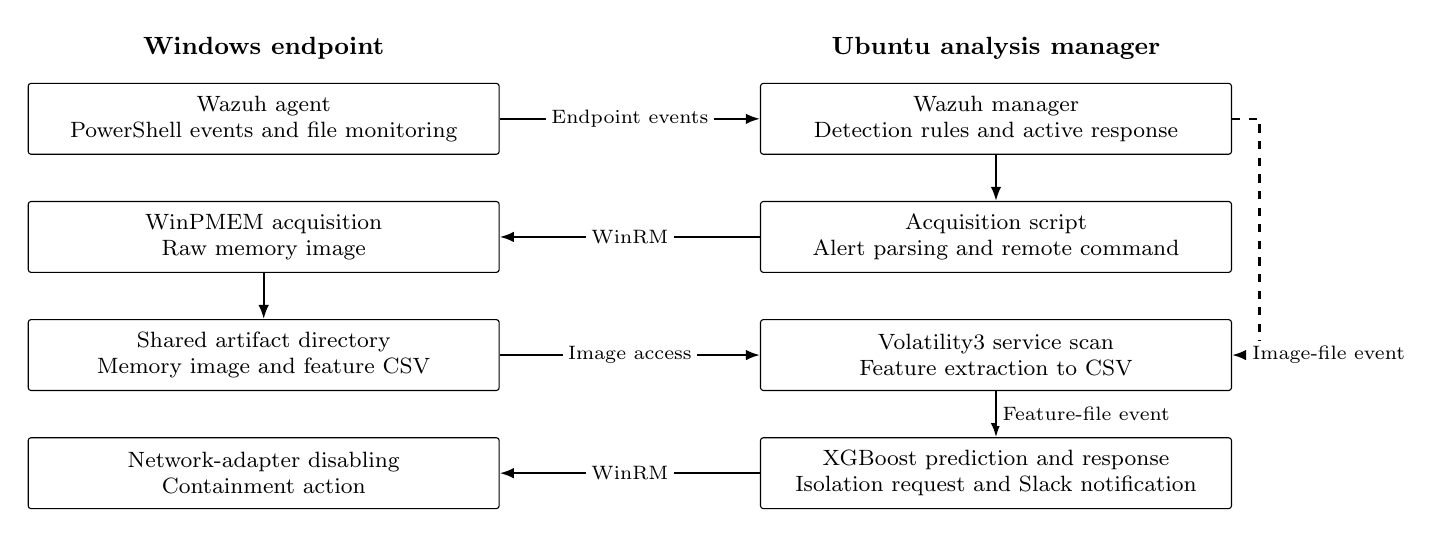
\begin{tikzpicture}[
  stage/.style={draw,rounded corners=1pt,align=center,
    text width=5.7cm,minimum height=0.9cm,inner sep=4pt,font=\footnotesize},
  flow/.style={-{Latex[length=1.8mm]},thick},
  note/.style={font=\scriptsize,fill=white,inner sep=2pt,align=center}]
\node[font=\small\bfseries] at (0,0.9) {Windows endpoint};
\node[font=\small\bfseries] at (9.3,0.9) {Ubuntu analysis manager};
\node[stage] (agent) at (0,0) {Wazuh agent\\PowerShell events and file monitoring};
\node[stage] (rules) at (9.3,0) {Wazuh manager\\Detection rules and active response};
\node[stage] (capture) at (0,-1.5) {WinPMEM acquisition\\Raw memory image};
\node[stage] (acquire) at (9.3,-1.5) {Acquisition script\\Alert parsing and remote command};
\node[stage] (share) at (0,-3) {Shared artifact directory\\Memory image and feature CSV};
\node[stage] (extract) at (9.3,-3) {Volatility3 service scan\\Feature extraction to CSV};
\node[stage] (isolate) at (0,-4.5) {Network-adapter disabling\\Containment action};
\node[stage] (response) at (9.3,-4.5) {XGBoost prediction and response\\Isolation request and Slack notification};
\draw[flow] (agent) -- node[note] {Endpoint events} (rules);
\draw[flow] (rules) -- (acquire);
\draw[flow] (acquire) -- node[note] {WinRM} (capture);
\draw[flow] (capture) -- (share);
\draw[flow] (share) -- node[note] {Image access} (extract);
\draw[flow] (extract) -- node[note,right] {Feature-file event} (response);
\draw[flow] (response) -- node[note] {WinRM} (isolate);
\draw[flow,dashed] (rules.east) -- ++(0.35,0) |- node[note,pos=0.75,right] {Image-file event} (extract.east);
\end{tikzpicture}
\caption{System architecture and principal stage transitions. Wazuh file events
initiate analysis and response; the shared directory provides the artifact
handoff. The manager sends the Slack notification after requesting isolation.}
\label{fig:architecture}
\end{figure*}

\subsection{Alert-Driven Memory Acquisition}
The Wazuh agent collects the Windows PowerShell operational log. Custom rules were configured to match indicators such as encoded-command execution and known offensive cmdlets. The active response script that triggers memory dump acquisition on the monitored host is configured with selected rule identifiers and a severity setting of 10. This stage uses the endpoint alert as a trigger to dump the monitored host's memory, and the subsequent classification is based on features extracted from the captured memory image.

The acquisition script reads the Wazuh JSON alert from standard input and extracts the agent name and address. It then invokes NetExec over WinRM to launch the preinstalled WinPMEM executable on that endpoint. The raw image is written to the configured dump path, and command output is appended to the acquisition log. Reading the target address from the alert connects the collection request to the endpoint that produced the triggering event.

The shared directory links the Windows acquisition path to the manager's analysis path. 
% Its use allows the analysis utilities to run on the manager while WinPMEM operates on the endpoint. 
This prototype uses fixed image and feature filenames suitable for the single-endpoint experiment. Concurrent incidents would require separate artifact locations and identifiers.

\subsection{Artifact-Based Stage Transitions}
Wazuh file-integrity monitoring (FIM) connects the acquisition and analysis stages. The recorded configuration associates raw-image events with extraction rules 100100/100101 and feature-file events with response rules 100102/100103. The next stage is consequently invoked by an observable file event rather than an analyst launching another tool. Table~\ref{tab:interfaces} summarizes
the interfaces.

\begin{table}[t]
\caption{Implemented Stage Interfaces}
\label{tab:interfaces}
\centering
\footnotesize
\begin{tabular}{@{}p{1.45cm}p{2.85cm}p{3.55cm}@{}}
\toprule
Stage & Input or trigger & Output or action \\
\midrule
Acquisition & Wazuh alert JSON & WinRM invocation; raw memory image \\
Extraction & Image-file FIM event & Volatility service records; feature CSV \\
Prediction & Feature CSV & Class label and model score in JSON \\
Response & Feature-file FIM event and prediction & Remote isolation request; Slack message \\
\bottomrule
\end{tabular}
\end{table}

The artifact interfaces also make individual stages inspectable. The raw image is the input to forensic analysis, the CSV records what the model receives, and the prediction message records the decision consumed by the response script. This separation provides a practical place to replace the extractor or decision component while retaining the surrounding workflow.

In the prototype, a file modification serves as the handoff signal. Such an event does not by itself prove that a large image has finished writing. The case study demonstrates a successful sequence; explicit completion markers, atomic publication of completed files, and duplicate-event handling are requirements for a more general implementation.

\subsection{Feature Extraction and Decision Interface}
The extraction script executes Volatility3's service-scan plugin using its JSON renderer. From the returned service records, it computes the total number of records and the number of distinct nonzero process identifiers associated with those records. These values are written as \texttt{svcscan.nservices} and \texttt{svcscan.process\_services}, in the column order expected by the classifier. The implementation uses a single plugin for the deployed decision path, keeping the feature interface compact.

The prediction script loads an XGBoost model and its associated standardization transform from a saved model bundle. The training notebook fits the scaler on the training partition and exports it with the classifier; inference applies that saved transform before prediction. The original two-feature experiment used a 70/30 split of the cleaned CIC-MalMem-2022 data and reported 99.84\% accuracy. Its operational interpretation is examined in Section~\ref{sec:assessment}.

The current prediction interface returns JSON containing the numeric label, class name, and malicious-class model score. The response script parses this message and follows the malicious branch when the numeric label equals one. The score is included in the analyst notification; it is not a separately calibrated response threshold. A benign prediction leaves the endpoint unchanged. If prediction output cannot be parsed, the current wrapper reports the problem and returns without issuing a response action.

\subsection{Containment, Notification, and Observability}
For a malicious prediction, the manager first requests network isolation over WinRM. The implemented PowerShell command enumerates the endpoint's network adapters and disables them. This action is intended to interrupt the endpoint's network communication, including its management connection. The manager then posts a Slack message containing the affected host, predicted class, and model score. Sending the notification from the manager allows it to occur after the endpoint's adapters have been disabled.

WinRM credentials and the Slack webhook are supplied through environment variables in the current scripts. The prototype records acquisition commands, feature-extraction progress, prediction results, and response activity. These records allow the case-study sequence to be reconstructed, although a success message from a command wrapper is not equivalent to independently verifying its effect. The subsequent connectivity observation provides additional response evidence in Section~\ref{sec:case}.

\section{Application Case Study: WannaCry Response}
\label{sec:case}

\subsection{Testbed and Evaluation Scope}
The functional evaluation uses a Windows 10 VM as the monitored endpoint and an Ubuntu VM as the Wazuh and analysis manager in an isolated virtual testbed. The configuration includes PowerShell event collection, a monitored shared artifact directory, preinstalled WinPMEM, and WinRM access for acquisition and response. WannaCry was introduced through a PowerShell download-and-execution sequence from a server within the testbed.

The evaluation asks whether the components execute the intended workflow: whether an endpoint event initiates acquisition, the image reaches extraction, the features reach classification, and the malicious branch invokes response and notification. Evidence consists of the recorded Wazuh events, script logs, and post-response connectivity observation. This is a single application demonstration, not a repeated trial of detection rates or response latency.

\subsection{Observed Workflow Execution}
The triggering activity initiated the acquisition script on the manager. Its log records the remote WinRM invocation and WinPMEM image generation. The subsequent extraction log records service-scan execution and successful feature extraction. Wazuh records the raw-image modification and the later feature-file modification under the configured FIM rules, linking the artifacts to their respective active responses.

The response log contains a malicious prediction, an isolation request, and a successful Slack-notification message (Fig.~\ref{fig:response}). A separate endpoint connectivity test records four unsuccessful probes to the manager, with local transmit failures. This is consistent with the adapter-disabling action and provides evidence beyond the response script's status message. It does not establish that every communication path was tested.

\begin{figure*}[t]
\centering
\includegraphics[width=\textwidth]{response_execution.png}
\caption{Recorded prediction and response stage in the WannaCry demonstration. The historical log shows the malicious decision, isolation request, and Slack notification. Its displayed model score describes this decision and is not a measured detection rate.}
\label{fig:response}
\end{figure*}

The demonstrated integration completes the operational sequence: an alert leads to an acquired image, the image produces a feature record, and the record drives a response decision. Table~\ref{tab:observations} relates the observations to the system objectives. The current scripts use a JSON decision message; the historical screenshot reflects the earlier dictionary-style serialization of the same decision fields.

\begin{table}[t]
\caption{Functional Evidence from the Application Case Study}
\label{tab:observations}
\centering
\footnotesize
\begin{tabular}{@{}p{2.5cm}p{5.55cm}@{}}
\toprule
Objective & Recorded observation \\
\midrule
Alert-driven collection & Acquisition script and remote WinPMEM execution \\
Automated analysis & Image FIM event; successful service-scan and feature-extraction messages \\
Decision handoff & Feature-file FIM event; malicious prediction consumed by response \\
Containment and notification & Isolation request; failed endpoint connectivity probes; Slack delivery reported \\
\bottomrule
\end{tabular}
\end{table}

\subsection{Recorded Timing}
Table~\ref{tab:timing} reports the available script-start timestamps from the
same run. Acquisition starts at 23:44:09, extraction at 23:45:09, and response
at 23:47:00, giving an acquisition-to-response initiation interval of 171\,s.
The 60\,s and 111\,s intervals separate stage starts; they include the work
and orchestration between those observations and are not isolated processing
benchmarks.

\begin{table}[t]
\caption{Recorded Stages11}
\label{tab:timing}
\centering
\small
\begin{tabular}{@{}lrr@{}}
\toprule
Stage & Start time & Elapsed from acquisition \\
\midrule
Acquisition & 23:44:09 & 0\,s \\
Feature extraction & 23:45:09 & 60\,s \\
Prediction and response & 23:47:00 & 171\,s \\
\bottomrule
\end{tabular}
\end{table}

The logs do not separately timestamp the initial suspicious activity or
completed containment. We therefore report the observed interval without
interpreting it as a full detection-to-containment latency. Repeated
measurements across memory sizes, workloads, and concurrent endpoints are
needed to characterize performance beyond this run.

\section{Supporting Assessment of the Decision Component}
\label{sec:assessment}

\subsection{Classifier Portability}
The working workflow makes the classifier's decision consequential: a positive
label can disable a host's network access. We therefore examined the public
training data as a supporting check on deployment readiness. CIC-MalMem-2022
contains 58{,}596 balanced records and 55 numeric features~\cite{carrier2022,cicmalmem}.
An ablation retains 52 nonconstant predictors and trains XGBoost models with
200 estimators, maximum depth 6, and a stratified 70/30 split with seed 7.
Training-partition scaling is used throughout.

The full feature set reaches 99.99\% accuracy, six host-configuration counters
reach 99.98\%, and the two-service-feature model reaches 99.84\%.
A descriptive rule using only service count, classifying values at most 391
or above 1000 as malicious, reaches 99.63\% on the full corpus. This last
result is not a held-out comparison. These findings show why high benchmark
accuracy alone is insufficient to establish sensitivity to malware on a
different endpoint.

Additional distribution checks reinforce the portability concern. All 22
selected count and count-derived indicators have higher benign medians, and
one-to-one load matching retains only 148 records. Five-fold logistic
regression assigns only 0.92\% of records to the intermediate probability band
$0.1<P(\mathrm{malicious}\mid x)<0.9$. This measures polarized class
predictions, not the causal effect of capture conditions. The dataset's
reported SMOTE augmentation also creates a risk of dependencies across random
partitions~\cite{carrier2022}; original/synthetic provenance is unavailable
to quantify that risk. For the system, the implication is to validate the
classifier on deployment-representative captures before allowing its label to
control containment.

\subsection{Host-Relative Scoring Extension}
As a candidate extension to the decision component, we implemented a
baseline-differential scorer fitted to clean captures from the same host.
An expanded extractor aggregates 44 features from eight Volatility3 plugins.
For feature $i$, let $m_i$ be its clean-reference median and $d_i$ its median
absolute deviation multiplied by 1.4826. The scorer computes
\begin{equation}
z_i(x)=\frac{x_i-m_i}{s_i+10^{-9}},\qquad
S_F(x)=\max_{i\in F}|z_i(x)|,
\end{equation}
where $s_i=d_i$ unless $d_i<10^{-6}$, in which case
$s_i=\max(0.01|m_i|,1)$. This representation makes deviation from a host's
reference state available to the decision stage. It has been evaluated
separately and is not integrated into the demonstrated containment path.

A small cloud pilot uses Atomic Red Team~\cite{atomicredteam} tests associated
with MITRE ATT\&CK T1055.001, .002, .003, .004, and .012~\cite{mitre1055} on
one Windows Server 2022 VM. Ten pre/post pairs were collected sequentially
within one boot session. A persistent shift in aggregate
\texttt{malfind.commitCharge}, from 259--265 in the first six pre-test captures
to 773--778 in the remaining four, led us to retain the first six pairs.
The shift is consistent with residual state after incomplete cleanup;
aggregate features do not establish the responsible process.

A restriction to 11 \texttt{malfind} and \texttt{ldrmodules} features gives
scores of 0.797 to 3.000 across the APC-injection pair and 4.000 to 5.000
across the process-hollowing pair. None of the six retained post-test captures
reaches the default threshold of 6. Using all 44 features flags three
post-test captures and one reference capture. The same six pre-test captures
fit the references, so these results do not estimate an independent
false-positive rate. The pilot establishes requirements for baseline coverage
and integrity rather than a validated replacement detector. Its feature
records and scoring implementation are retained for further evaluation.

\section{Discussion and Deployment Requirements}
\label{sec:discussion}

\subsection{Application Value and Design Tradeoffs}
The case study demonstrates that an endpoint alert can initiate memory
collection and carry its output through analysis to a response action. For an
analyst, the resulting workflow provides a captured image, an explicit feature
record, and a decision associated with the affected endpoint. These artifacts
support subsequent investigation even when the classifier itself requires
further validation. The integration removes manual stage invocation in the
demonstrated sequence; analyst-time savings were not measured.

The main operational tradeoff is acquisition before containment. Keeping the
management and shared-folder paths available permits the forensic workflow to
complete, while the suspect host remains connected during collection and
analysis. A deployment must choose the order of collection and containment
according to its incident policy and available management paths. The current
prototype implements collection first.

\subsection{Reliability and Scope}
Generalizing the implementation requires explicit state at the stage boundaries:
a completed-image signal, incident-specific filenames, suppression of duplicate
FIM triggers, and confirmation that a response command achieved its intended
effect. The current isolation wrapper does not check the remote command's exit
status before printing success. Recorded connectivity loss supports the case
study, while routine deployment would require a separate verification step.
These are engineering requirements arising from the implemented workflow.

The evaluation covers one Windows endpoint and one WannaCry demonstration.
It does not establish concurrent throughput, recovery behavior, detection
coverage across malware families, or a containment-latency distribution. The
supporting pilot also uses a single host image, couples workload and technique
in a fixed rotation, and lacks retained raw images and per-test execution
transcripts. Its results guide feature and baseline design without substituting
for a larger system evaluation. Future work will combine repeated functional
tests, independent classifier calibration, and verified recovery from failed
acquisition or response stages.

\section{Conclusion}

We presented an automated memory-forensics system that integrates Wazuh alerts,
WinPMEM acquisition, Volatility3 analysis, XGBoost classification, and remote
containment with analyst notification. The Windows--Ubuntu implementation
connects these components through active-response rules, shared artifacts,
and structured decision messages. A WannaCry case study demonstrates the
workflow, with recorded acquisition, analysis, response, and connectivity
observations; script-start timestamps show 171\,s from acquisition initiation
to response initiation.

The supporting classifier audit and host-relative pilot identify requirements
for deploying the decision component across different environments. The next
step is to strengthen stage-completion and response verification, evaluate
multiple endpoints and workloads, and calibrate the decision policy with
independent captures. These extensions build on the demonstrated integration
of forensic collection and automated incident response.

\begin{thebibliography}{10}
\bibitem{wazuh} Wazuh, ``Active Response,'' \textit{Wazuh Documentation}.
Accessed: Sep. 9, 2026. [Online]. Available:
\url{https://documentation.wazuh.com/current/user-manual/capabilities/active-response/index.html}

\bibitem{winpmem} Velocidex, ``WinPmem: A Physical Memory Acquisition Tool.''
Accessed: Sep. 9, 2026. [Online]. Available:
\url{https://github.com/Velocidex/WinPmem}

\bibitem{volatility} Volatility Foundation, ``Volatility 3 Documentation.''
Accessed: Sep. 9, 2026. [Online]. Available:
\url{https://volatility3.readthedocs.io/en/latest/}

\bibitem{lashkari2021} A. H. Lashkari, B. Li, T. L. Carrier, and G. Kaur,
``VolMemLyzer: Volatile Memory Analyzer for Malware Classification using
Feature Engineering,'' in \textit{Proc. Reconciling Data Analytics,
Automation, Privacy, and Security: A Big Data Challenge (RDAAPS)},
2021, pp. 1--8, doi: 10.1109/RDAAPS48126.2021.9452028.

\bibitem{carrier2022} T. Carrier, P. Victor, A. Tekeoglu, and A. H. Lashkari,
``Detecting Obfuscated Malware using Memory Feature Engineering,'' in
\textit{Proc. 8th Int. Conf. Information Systems Security and Privacy
(ICISSP)}, 2022, pp. 177--188, doi: 10.5220/0010908200003120.

\bibitem{arp2022} D. Arp, E. Quiring, F. Pendlebury, A. Warnecke,
F. Pierazzi, C. Wressnegger, L. Cavallaro, and K. Rieck,
``Dos and Don'ts of Machine Learning in Computer Security,'' in
\textit{Proc. 31st USENIX Security Symp.}, 2022, pp. 3971--3988.

\bibitem{cicmalmem} Canadian Institute for Cybersecurity,
``Malware Memory Analysis (CIC-MalMem-2022),'' University of New Brunswick.
Accessed: Sep. 9, 2026. [Online]. Available:
\url{https://www.unb.ca/cic/datasets/malmem-2022.html}

\bibitem{atomicredteam} Red Canary, ``Atomic Red Team.''
Accessed: Sep. 9, 2026. [Online]. Available:
\url{https://github.com/redcanaryco/atomic-red-team}

\bibitem{mitre1055} MITRE, ``Process Injection, Technique T1055,''
\textit{MITRE ATT\&CK}.
Accessed: Sep. 9, 2026. [Online]. Available:
\url{https://attack.mitre.org/techniques/T1055/}

\end{thebibliography}
\end{document}
